\documentclass[oneside,letterpaper,12pt]{book}
\usepackage{bibentry}
\usepackage{graphicx}
\usepackage{natbib}
\usepackage[reqno]{amsmath}
\usepackage{amssymb}
\usepackage{verbatim}
\usepackage{epsf}
\usepackage{url}
\usepackage{html}
\usepackage{dcolumn}
\usepackage{fullpage}
\bibpunct{(}{)}{;}{a}{}{,}
\newcolumntype{.}{D{.}{.}{-1}}
\newcolumntype{d}[1]{D{.}{.}{#1}}
%\pagestyle{myheadings}
\htmladdtonavigation{
  \htmladdnormallink{%
    \htmladdimg{http://gking.harvard.edu/pics/home.gif}}
  {http://gking.harvard.edu/}}
\newcommand{\hlink}{\htmladdnormallink}

%\bodytext{ BACKGROUND="http://gking.harvard.edu/pics/temple.jpg"}
\setcounter{tocdepth}{3}
\setcounter{secnumdepth}{4}

\newcommand{\MatchIt}{\textsc{MatchIt}}

\title{\MatchIt: Nonparametric Preprocessing for Parametric Causal
  Inference\thanks{We thank Olivia Lau for helpful suggestions about
    incorporating \MatchIt\, into Zelig.}}

\author{Daniel E. Ho,\thanks{Assistant Professor of Law 
\& Robert E.\ Paradise Faculty Scholar, Stanford Law
    School (559 Nathan Abbott Way, Stanford CA 94305;
    \texttt{http://dho.stanford.edu}, \texttt{dho@law.stanford.edu},
    (650) 723-9560).}  \and %
  Kosuke Imai,\thanks{Assistant Professor, Department of Politics,
    Princeton University (Corwin Hall 041, Department of Politics,
    Princeton University, Princeton NJ 08544, USA;
    \texttt{http://imai.princeton.edu},
    \texttt{kimai@Princeton.Edu}).}  \and %
  Gary King,\thanks{David Florence Professor of Government, Harvard
    University (Institute for Quantitative Social Science, 1737
    Cambridge Street, Harvard University, Cambridge MA 02138;
    \texttt{http://GKing.Harvard.Edu}, \texttt{King@Harvard.Edu},
    (617) 495-2027).}  \and %
Elizabeth A. Stuart\thanks{Assistant Professor, Departments of Mental 
Health and Biostatistics, Johns Hopkins Bloomberg School of Public Health 
(624 N Broadway, Room 804, Baltimore, MD 21205; 
  \texttt{http://www.biostat.jhsph.edu/$\sim$estuart},
  \texttt{estuart@jhsph.edu}).}}

%\makeindex

\begin{document}
\maketitle

\begin{rawhtml}
  <p> [Also available is a downloadable <a
  href="matchit.pdf">PDF</a> version of this entire
  document]
\end{rawhtml}

\tableofcontents

\nobibliography*

%%%%%%%%%%%%%%%%%%%%%%%%%%%%%%%%%%%%%%%%%%%%%%%%%%%%%%%%%%%%%%%%%%%%%%%%
\clearpage

\chapter{Introduction}

\section{What \MatchIt\ Does}

\MatchIt\ implements the suggestions of \citet*{HoImaKin05} for
improving parametric statistical models and reducing model dependence
by preprocessing data with semi-parametric and non-parametric matching
methods.  After preprocessing with \MatchIt, researchers can use
whatever parametric model and software they would have used without
\MatchIt, without other modification, and produce inferences that are
substantially more robust and less sensitive to modeling assumptions.
(In addition, you may wish to use
\hlink{Zelig}{http://gking.harvard.edu/zelig/} \citep{ImaKinLau04} for
subsequent parametric analyses, as it is designed for maximum
convenience in analyzing \MatchIt\ datasets.)  \MatchIt\ reduces the
dependence of causal inferences on commonly made, but hard-to-justify,
statistical modeling assumptions via a wide range of sophisticated
matching methods.  In addition, we have written \MatchIt\ so that
adding new matching methods to the software is as easy for anyone with
the inclination as it is for us.

\section{Software Requirements} 
\label{sec:require}

\MatchIt\ works in conjunction with the R programming language and
statistical software, and will run on any platform where R is
installed (Windows, Unix, or Mac OS X).  R is available free for
download at the Comprehensive R Archive Network (CRAN) at
\hlink{http://cran.r-project.org/}{http://cran.r-project.org/}.
\MatchIt\ has been tested on the most recent version of R.  A good way
to learn R, if you don't know it already, is to learn Zelig (available
at \hlink{http://gking.harvard.edu}{http://gking.harvard.edu}) which
includes a self-contained introduction to R and can be used to analyze
the matched data after running \MatchIt.

\section{Installing \MatchIt}
\label{sec:install}

To install \MatchIt\ for all platforms, type at the R command prompt,
\begin{verbatim}
> install.packages("MatchIt")
\end{verbatim}
and \MatchIt\ will install itself onto your system automatically.
During the installation process you may either decide to keep or
discard the installation files, which will not affect the way
\MatchIt\ runs.  Note that you only need to do this once.  
%Some users
%may also find it helpful to install the package with version control
%(see Subsection~\ref{subsec:vercontrol}). 
We recommend that users also install Zelig, Matching, and optmatch by
typing the following commands,
\begin{verbatim}
> install.packages("Zelig")
> install.packages("Matching")
> install.packages("optmatch", contriburl = "http://www.stat.lsa.umich.edu/~bbh/optmatch")
\end{verbatim}


\section{Loading \MatchIt} \label{sec:load}

As with any R package, you need install \MatchIt\ only once, but you
must load it prior to each use.  You can do this for each R session by
typing,
\begin{verbatim}
> library(MatchIt)
\end{verbatim}
at the R command prompt.  

Alternatively, you can specify R to load \MatchIt\ automatically at
launch so that you can skip the step of typing {\tt library(MatchIt)}
at the beginning of every R session.  To do this, edit the {\tt
  Rprofile} file located in the R program subdirectory, e.g.
\texttt{C:/R/rw2011/etc/}, for Windows systems or the {\tt .Rprofile}
file located in the home directory for Unix/Linux and Mac OS X
systems.  Using a text editor such as Windows notepad and emacs, add
the following line to the file,
\begin{verbatim}
options(defaultPackages = c(getOption("defaultPackages"), "MatchIt"))
\end{verbatim}
For this change to take effect, you need to restart R.

\section{Updating \MatchIt}

We recommend that you periodically update \MatchIt\ at the R prompt by typing:
\begin{verbatim}
> update.packages()
> library(MatchIt)
\end{verbatim}
which will update all the libraries including \MatchIt\ and load the
new version of \MatchIt.


%%% Local Variables: 
%%% mode: pdflatex
%%% TeX-master: "matchit"
%%% End: 



%%%%%%%%%%%%%%%%%%%%%%%%%%%%%%%%%%%%%%%%%%%%%%%%%%%%%%%%%%%%%%%%%%%%%%%%

\chapter{Statistical Overview}

\MatchIt\ is designed for studies with a dependent variable (or a set
of dependent variables) that is a function of a dichotomous causal (or
``treatment'') variable, with values known as the ``treated'' and
``control'' groups, and a set of ``pretreatment'' covariates, i.e.,
that are causally prior to the administration of the treatment.  (If
you are interested in the causal effect of more than one variable in
your data set, run \MatchIt\ separately for each one; it is unlikely
in any event that any one parametric model will produce valid causal
inferences for more than one treatment variable at a time.)  \MatchIt\
can be used for other types of causal variables by dichotomizing them,
perhaps in multiple ways \citep[see also][]{ImaDyk04}.  \MatchIt\
works for experimental data, but is designed mainly for observational
studies where the treatment variable is simply observed rather than
manipulated at will by the investigator.

We adopt the same notation as in \citet*{HoImaKin05}. Unless otherwise
noted, let $i$ index the $n$ units in the dataset, $n_1$ denote the
number of treated units, $n_0$ denote the number of control units
(such that $n=n_0+n_1$), and $x_i$ indicate a vector of pretreatment
(or control) variables for unit $i$.  Let $t_i=1$ when unit $i$ is
assigned treatment, and $t_i=0$ when unit $i$ is assigned control.
(The labels ``treatment'' and ``control'' are arbitrary and can be
switched for convenience.)  Denote $y_i(1)$ as the potential outcome
of unit $i$ under treatment --- the value the outcome variable would
take if $t_i$ were equal to 1, whether or not $t_i$ in fact is 0 or 1
-- and $y_i(0)$ the potential outcome of unit $i$ under control ---
the value the outcome variable would take if $t_i$ were equal to 0,
regardless of its value in fact.  The variables $y_i(1)$ and $y_i(0)$
are jointly unobservable, and for each $i$, we observe one
$y_i=t_iy_i(1)+(1-t_i)y_i(0)$, and not the other.

\section{Preprocessing via Matching}

If $t_i$ and $X_i$ were independent, we would not need to control for
$X_i$, and any parametric analysis would effectively reduce to a
difference in means of $Y$ for the treated and control groups.  The
goal of matching is to preprocess the data prior to the parametric
analysis so that the actual relationship between $t_i$ and $X_i$ is
eliminated or reduced without introducing bias and inefficiency.  When
matching we select, duplicate, or selectively drop observations from
our data, and we do so without inducing bias as long as we use a rule
that is a function only of $t_i$ and $X_i$ and does not depend on the
outcome variable $Y_i$.  \MatchIt\ implements and evaluates the choice
of these rules.  

The simplest way to obtain good matches (as defined above) is to use
one-to-one exact matching, which pairs each treated unit with one
control unit for which the values of $X_i$ are identical.  However,
with many covariates and finite numbers of potential matches, it is
often very difficult to obtain exact matches.  Fortunately, good
matching only requires that the empirical \emph{distribution} of $X$
given $t=0$ match that of $X$ given $t=1$, and so individual (exactly)
matched pairs are not required.  Formally the goal of matching is
$\tilde p(X\mid t=1) \approx \tilde p(X\mid t=0)$, where $\tilde p$
refers to the observed empirical density of the data (think
histogram), rather than a population density.  Indeed, many of the
other methods implemented in \MatchIt\ only attempt to balance the
overall covariate distributions, without necessarily finding
one-to-one exact matches.

A key point in \citet*{HoImaKin05} is that matching methods by
themselves are not methods of estimation: Every use of matching in the
literature involves an analysis step following the matching procedure,
but almost all analyses use a simple difference in means.  This
procedure is appropriate only if exact matching was conducted.  In
almost all other cases, some adjustment is required, and there is no
reason to degrade your inferences by using an inferior method of
analysis such as a difference in means even when improving your
inferences via preprocessing.  Thus, with \MatchIt, you can improve
your analyses in two ways.  In fact, \MatchIt\ analyses are ``doubly
robust'' in that if \emph{either} the matching analysis or the
analysis model is correct (but not necessarily both) your inferences
will be statistically consistent.

\section{Checking Balance}
\label{sec:balance-sum}

The goal of matching is to create a data set that looks closer to one
that would result from a randomized experiment.  When we get close, we
break the link between treatment variable and the pretreatment
controls, which makes the parametric form of the analysis model less
relevant or irrelevant entirely.  To break this link, we need the
distribution of covariates to be the same within the matched treated
and control groups.

A crucial part of any matching procedure is, therefore, to assess how
close the (empirical) covariate distributions are in the two groups,
which is known as ``balance.''  Because the outcome variable is not
used in the matching procedure, a variety of matching methods can be
assessed, and the matching procedure that leads to the best balance is
chosen.  \MatchIt\ provides a number of ways to assess the balance of
covariates after matching, including numerical summaries such as the
bias (difference in means) or standardized bias (difference in means
divided by the treated group standard deviation), and graphical
summaries such as quantile-quantile plots that compare the empirical
distributions of each covariate, and numerical summaries of this
graphical summary.  The widely used procedure of doing t-tests of the
difference in means is highly misleading and should never be used to
assess balance.  These diagnostics can be done on all the covariates
that are included in the matching procedure, as well as on other
covariates on which close matches are desired.

\section{Conducting Analyses after Matching}

The most common way that parametric analyses are used to compute
quantities of interest (without matching) is by holding constant some
explanatory variables, changing others, and computing predicted or
expected values and taking the difference or ratio, all by using the
parametric functional form.  In the case of causal inference, this
would mean looking at the effect on the expected value of the outcome
variable when changing $T$ from 0 to 1, while holding constant the
pretreatment control variables $X$ at their means or medians.  This,
and indeed any other standard procedure, would be a perfectly
reasonable way to proceed with analysis after matching.

Another increasingly popular way to proceed with analysis after
\MatchIt\ is to compute the \emph{average treatment effect on the
  treated}.  For example, for the treated group, the potential
outcomes under control, $Y_i(0)$, are missing, whereas the outcomes
under treatment, $Y_i(1)$, are observed, and the goal of the analysis
is to impute the missing outcomes, $Y_i(0)$ in observations where
$T_i=1$.  We do this via simulation using a parametric statistical
model (as described below).  Once those potential outcomes are imputed
from the model, the estimate of individual $i$'s treatment effect is
$Y_i(1)-\widehat{Y}_i(0)$ where $\widehat{Y}_i(0)$ is a Monte Carlo
estimate of the average missing potential outcome for unit $i$ (i.e.,
the average of simulated values of the dependent variable for unit $i$
under the counterfactual condition where $T_i=0$).  The in-sample
average treatment effect for the treated individuals can then be
obtained by averaging this difference over all observations $i$ where
in fact $T_i=1$.  (A similar procedure can also be used to estimate
various other quantities of interest such as the average treatment
effect for all observations.)  An advantage of this simulation
approach is that the uncertainty estimates such as standard errors and
confidence intervals are obtained easily by the usual rules in fitting
the parametric model.

The imputation from the model can be done in at least two ways.
Recall that the model is used to impute \emph{the value that the
  outcome variable would take among the treated units if those treated
  units were actually controls}.  Thus, one reasonable approach would
be to fit a model to the matched data and create simulated predicted
values of the dependent variable for the treated units with $T_i$
switched counterfactually from 1 to 0.  An alternative approach would
be to fit a model without $T$ by using only the outcomes of the
matched control units (i.e., using only observations where $T_i=0$).
Then, given this fitted model, the missing outcomes $Y_i(0)$ are
imputed for the matched treated units by using the values of the
explanatory variables for the treated units.  The first approach will
usually have lower variance, since all observations are used, and the
second may have less bias, since no assumption of constant parameters
is needed.  See \citet*{HoImaKin05} for more details.

% Local Variables: 
%%% mode: latex
%%% TeX-master: "matchit"
%%% End: 


%%%%%%%%%%%%%%%%%%%%%%%%%%%%%%%%%%%%%%%%%%%%%%%%%%%%%%%%%%%%%%%%%%%%%%%%%%%

\chapter{User's Guide to \MatchIt}
\label{methods}

\section{Preprocessing via Matching}
\label{sec:matching}

\subsection{Quick Overview}

The main command \texttt{matchit()} implements the matching
procedures.  A general syntax is:
\begin{verbatim}
> m.out <- matchit(treat ~ x1 + x2, data = mydata)
\end{verbatim}
where {\tt treat} is the dichotomous treatment variable, and {\tt x1}
and {\tt x2} are pre-treatment covariates, all of which are contained
in the data frame {\tt mydata}.  The dependent variable (or variables)
may be included in \texttt{mydata} for convenience but is never used
by \MatchIt\ or included in the formula.  This command creates the
\MatchIt\ object called \texttt{m.out}.  Name the output object to see
a quick summary of the results:
\begin{verbatim}
> m.out
\end{verbatim}

\subsection{Examples}

To run any of the examples below, you first must load the library and
and data:
\begin{verbatim}
> library(MatchIt)
> data(lalonde)
\end{verbatim}

Our example data set is a subset of the job training program analyzed
in \citet{lalonde86} and \citet{DehWah99}. \MatchIt\ includes a
subsample of the original data consisting of the National Supported
Work Demonstration (NSW) treated group and the comparison sample from
the Population Survey of Income Dynamics (PSID).\footnote{This data
  set, \texttt{lalonde}, was created using NSWRE74$\_$TREATED.TXT and
  CPS3$\_$CONTROLS.TXT from
  http://www.columbia.edu/$\sim$rd247/nswdata.}  The variables in this
data set include participation in the job training program
(\texttt{treat}, which is equal to 1 if participated in the program,
and 0 otherwise), age ({\tt age}), years of education ({\tt educ}),
race (\texttt{black} which is equal to 1 if black, and 0 otherwise;
\texttt{hispan} which is equal to 1 if hispanic, and 0 otherwise),
marital status (\texttt{married}, which is equal to 1 if married, 0
otherwise), high school degree (\texttt{nodegree}, which is equal to 1
if no degree, 0 otherwise), 1974 real earnings (\texttt{re74}), 1975
real earnings (\texttt{re75}), and the main outcome variable, 1978
real earnings (\texttt{re78}).

\subsubsection{Exact Matching}
\label{subsubsec:exact}

The simplest version of matching is exact.  This technique matches
\emph{each} treated unit to \emph{all} possible control units with
exactly the same value on all the covariates, forming subclasses such
that within each subclass all units (treatment and control) have the
same covariate values.  Exact matching is implemented in \MatchIt\ 
using \texttt{method = "exact"}.  Exact matching will be done on all
covariates included on the right-hand side of the \texttt{formula}
specified in the \MatchIt\ call.  There are no additional options for
exact matching.  (Exact restrictions on a subset of covariates can
also be specified in nearest neighbor matching; see
Section~\ref{subsubsec:nearest}.)  The following example can be
run by typing {\tt demo(exact)} at the R prompt,
\begin{verbatim}
> m.out <- matchit(treat ~ educ + black + hispan, data = lalonde, 
                   method = "exact")
\end{verbatim}

\subsubsection{Subclassification}
\label{subsubsec:subclass}

When there are many covariates (or some covariates can take a large
number of values), finding sufficient exact matches will often be
impossible.  The goal of subclassification is to form subclasses, such
that in each the distribution (rather than the exact values) of
covariates for the treated and control groups are are as similar as
possible.  Various subclassification schemes exist, including the one
based on a scalar distance measure such as the propensity score
estimated using the \texttt{distance} option (see
Section~\ref{subsubsec:inputs-all}).  Subclassification is implemented
in \MatchIt\ using \texttt{method = "subclass"}.

The following example script can be run by typing {\tt demo(subclass)}
at the R prompt,
\begin{verbatim}
> m.out <- matchit(treat ~ re74 + re75 + educ + black + hispan + age, 
                   data = lalonde, method = "subclass")
\end{verbatim}
The above syntax forms 6 subclasses, which is the default number
of subclasses, based on a distance measure estimated using logistic
regression.  By default, each subclass will have approximately the
same number of treated units.

Subclassification may also be used in conjunction with nearest
neighbor matching described below, by leaving the default of
\texttt{method = "nearest"} but adding the option \texttt{subclass}.
When you choose this command, \MatchIt\ matches in the same way, but
after the nearest neighbor matches are chosen it places them into
subclasses, and adds a variable to the output object with the subclass
numbers.

\subsubsection{Nearest Neighbor Matching}
\label{subsubsec:nearest}

Nearest neighbor matching selects the $r$ (default=1) best control
matches for each individual in the treatment group (excluding those
discarded using the \texttt{discard}) option.  The matching is done
using a distance measure specified by the {\tt distance} option
(default=logit).  Matches are chosen for each treated unit one at a
time, and at each matching step we choose the control unit that is not
yet matched but is closest to the treated unit on the distance
measure.

Nearest neighbor matching is implemented in \MatchIt\ using the
\texttt{method = "nearest"} option.  The following example script can
be run by typing {\tt demo(nearest)}:
\begin{verbatim}
> m.out <- matchit(treat ~ re74 + re75 + educ + black + hispan + age, 
                   data = lalonde, method = "nearest")
\end{verbatim}

\subsubsection{Optimal Matching}
\label{subsubsec:optimal}

The default nearest neighbor matching method in \MatchIt\ is
``greedy'' matching, where the closest control match for each treated
unit is chosen one at a time, without trying to minimize a global
distance measure.  In contrast, ``optimal'' matching finds the matched
samples with the smallest average absolute distance across all the
matched pairs.  \citet{GuRos93} find that greedy and optimal matching
approaches generally choose the same sets of controls for the overall
matched samples, but optimal matching does a better job of minimizing
the distance within each pair.  In addition, optimal matching can be
helpful when there are not many appropriate control matches for the
treated units.

Optimal matching is performed with \MatchIt\ by setting \texttt{method
  = "optimal"}, which automaticaly loads an add-on package called
\texttt{optmatch} \citep{Hansen04}.  The following example can also be
run by typing {\tt demo(optimal)} at the R prompt.  We conduct optimal
ratio matching based on the propensity score from the logistic
regression.
\begin{verbatim}
> m.out <- matchit(treat ~ re74 + re75 + age + educ, data = lalonde, 
                   method = "optimal", ratio = 2)
\end{verbatim}

\subsubsection{Full Matching}
\label{subsubsec:full}

Full matching is a a particular type of subclassification that uses
all treated and control units \citep{Rosenbaum02, Hansen04}.  A fully
matched sample is composed of matched sets, where each matched set
contains one treated unit and one or more controls (or one control
unit and one or more treated units).  The only units not placed into a
subclass will be those discarded (if a \texttt{discard} option is
specified) because they are outside the range of common support.  Full
matching is optimal in terms of minimizing a weighted average of the
estimated distance measure between each treated subject and each
control subject within each subclass.

Full matching can be performed with \MatchIt\ by setting
\texttt{method = "full"}.  We use an add-on package called
\texttt{optmatch} \citep{Hansen04}, which will be automatically
installed when needed.  The following example with full matching
(using the default propensity score based on logistic regression) can
also be run by typing {\tt demo(full)} at the R prompt:
\begin{verbatim}
> m.out <- matchit(treat ~ age + educ + black + hispan + married +
                   nodegree + re74 + re75, data = lalonde, method = "full")
\end{verbatim}

\subsubsection{Genetic Matching}
\label{subsub:genetic}

Genetic matching automates the process of finding a good matching
solution \citep{DiaSek05}.  The idea is to use a genetic search
algorithm to find a set of weights for each covariate such that the a
version of optimal balance is achieved after matching.  As currently
implemented, matching is done with replacement using the matching
method of \citet{AbaImb04} and balance is determined by two univariate
tests, paired t-tests for dichotomous variables and a
Kolmogorov-Smirnov test for multinomial and continuous variables, but
these options can be changed.

Genetic matching can be performed with \MatchIt\ by setting
\texttt{method = "genetic"}, which automatically loads the
\texttt{Matching} \citep{Sekhon04} package.  The following example of
genetic matching (using the estimated propensity score based on
logistic regression as one of the covariates) can also be run by
typing {\tt demo(genetic)}:
\begin{verbatim}
> m.out <- matchit(treat ~ age + educ + black + hispan + married + nodegree + 
                   re74 + re75, data = lalonde, method = "genetic")
\end{verbatim}


%%% Local Variables: 
%%% mode: latex
%%% TeX-master: "matchit"
%%% End: 

\section{Checking Balance}
\label{sec:balance}

\subsection{Quick Overview}

To check balance, use \texttt{summary(m.out)} for numerical summaries
and \texttt{plot(m.out)} for graphical summaries.

\subsection{Details}

\subsubsection{The {\tt summary()} Command}

The \texttt{summary()} command gives measures of the balance between
the treated and control groups in the full (original) data set, and
then in the matched data set.  If the matching worked well, the
measures of balance should be smaller in the matched data set (smaller
values of the measures indicate better balance).

The \texttt{summary()} output for subclassification is the same as
that for other types of matching, except that the balance statistics
are shown separately for each subclass, and the overall balance in the
matched samples is calculated by aggregating across the subclasses,
where each subclass is weighted by the number of units in the
subclass.  For exact matching, the covariate values within each
subclass are guaranteed to be the same, and so the measures of balance
are not output for exact matching; only the sample sizes in each
subclass are shown.

\begin{itemize}
\item {\bf Balance statistics:} The statistics the \texttt{summary()}
  command provides include means, the original control group standard deviation (where applicable), 
  mean differences, standardized mean
  differences, and (median, mean and maximum) Quantile-Quantile (Q-Q)
  plot differences.  In addition, the \texttt{summary()} command will
  report (a) the matched call, (b) how many units were matched,
  unmatched, or discarded due to the \texttt{discard} option
  (described below), and (c) the percent improvement in balance for
  each of the balance measures, defined as $100((|a|-|b|)/|a|)$, where
  $a$ is the balance before and $b$ is the balance after matching.
  For each set of units (original and matched data sets, with weights
  used as appropriate in the matched data sets), the
  following statistics are provided:
\begin{enumerate}
  \item ``Means Treated'' and ``Means Control'' show the weighted
    means in the treated and control groups
  \item ``SD Control" is the standard deviation calculated in the control group (where applicable)
  \item ``Mean Diff'' is the difference in means between the groups
  \item The final three columns of the summary output give summary
    statistics of a Q-Q plot (see below for more information on these
    plots). Those columns give the median, mean, and maximum distance
    between the two empirical quantile functions (treated and control
    groups).  Values greater than 0 indicate deviations between the
    groups in some part of the empirical distributions.  The plots of
    the two empirical quantile functions themselves, described below,
    can provide further insight into which part of the covariate
    distribution has differences between the two groups.
\end{enumerate}

\item {\bf Additional options:} Three options to the \texttt{summary()}
  command can also help with assessing balance and respecifying the
  propensity score model, as necessary.  First, the {\tt interactions
    = TRUE} option with {\tt summary()} shows the balance of all
  squares and interactions of the covariates used in the matching
  procedure.  Large differences in higher order interactions usually
  are a good indication that the propensity score model (the distance measure) needs to be
  respecified.  Similarly, the {\tt addlvariables} option with {\tt
    summary()} will provide balance measures on additional variables
  not included in the original matching procedure.  If a variable (or
  interaction of variables) not included in the original propensity score model
  has large imbalances in the matched groups, including that
  variable in the next model specification may improve the resulting
  balance on that variable.  Because the outcome variable is not used
  in the matching procedure, a variety of matching methods can be
  tried, and the one that leads to the best resulting balance chosen.  Finally,
  the {\tt standardize = TRUE} option will print out standardized versions of the
  balance measures, where the mean difference is standardized (divided) by the standard deviation
  in the original treated group.
\end{itemize}

\subsubsection{The \texttt{plot()} Command}

We can also examine the balance graphically using the \texttt{plot()}
command, which provides three types of plots: jitter plots of the
distance measure, Q-Q plots of each covariate, and histograms of the 
distance measure.  For subclassification, separate Q-Q plots are
printed for each subclass.  The jitter plot for subclassification is
the same as that for other types of matching, with the addition of
vertical lines indicating the subclass cut-points.  With the histogram option,
4 histograms are provided: the original treated and control groups and the matched
treated and control groups.  For the Q-Q plots and the histograms, the weights that result
after matching are used to create the plots.

%\begin{figure}[tbp]
%  \begin{center}
%    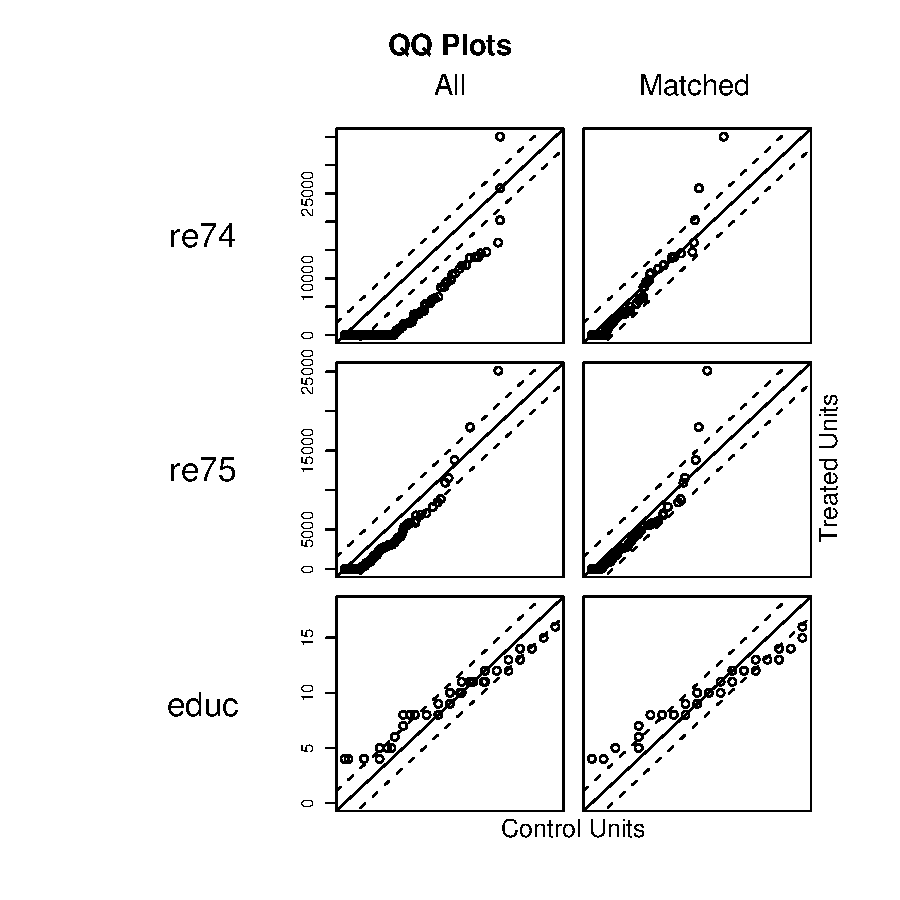
\includegraphics{figs/qqplotnn1}
%    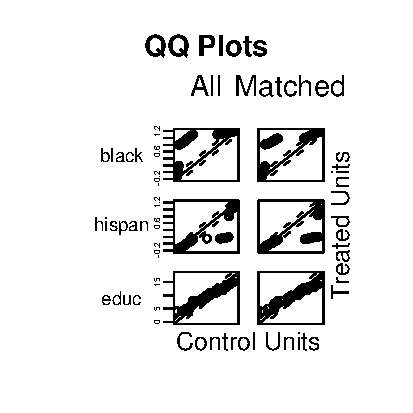
\includegraphics{figs/qqplotnn2}
%    \hfill
%    \caption{Sample diagnostic QQ plots with nearest neighbor matching}
%    \label{diagqqnn}
%  \end{center}
%\end{figure}

%\begin{figure}[tbp]
%  \begin{center}
%    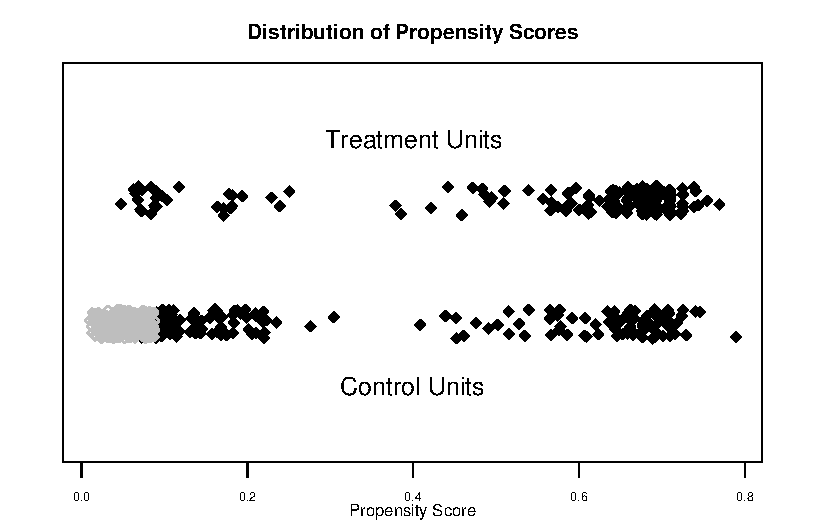
\includegraphics{figs/jitterplotnn}
%    \hfill
%    \caption{Sample diagnostic jitter plot: Matched units shown in
%      black, unmatched units shown in grey.}
%    \label{diagjitternn}
%  \end{center}
%\end{figure}

Three examples of the output from the {\tt plot()} command are shown
below.  If the empirical distributions are the same in the treated and
control groups, the points in the Q-Q plots would all lie on the 45 degree line.
Deviations from the 45 degree line indicate differences in the
empirical distribution.  The jitter plot shows the overall
distribution of propensity scores in the treated and control groups.
In the jitter plot, the size of each diamond is proportional to the
weight given to that unit; matched units are in black while unmatched
units are in grey. In the jitter
plot, which can be created by setting \texttt{type = "jitter"}, you
may identify units by observation name by clicking the first mouse
button near the units.  The histograms can be plotted by setting \texttt{type = "hist"}. 


\hspace{-0.75in}
\begin{center}
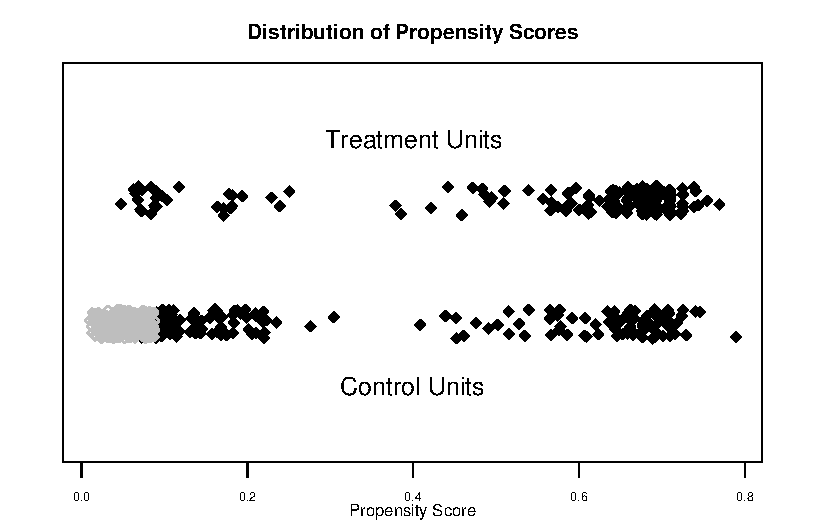
\includegraphics[height=3in]{figs/jitterplotnn}\\
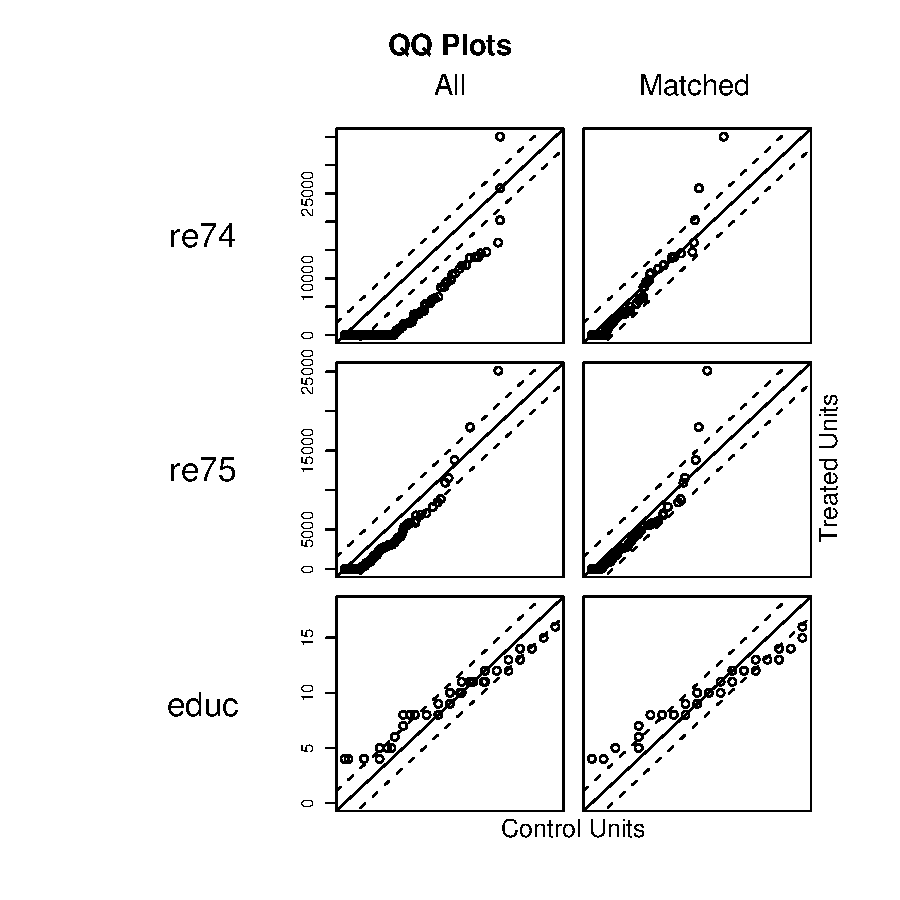
\includegraphics[height=3in]{figs/qqplotnn1}
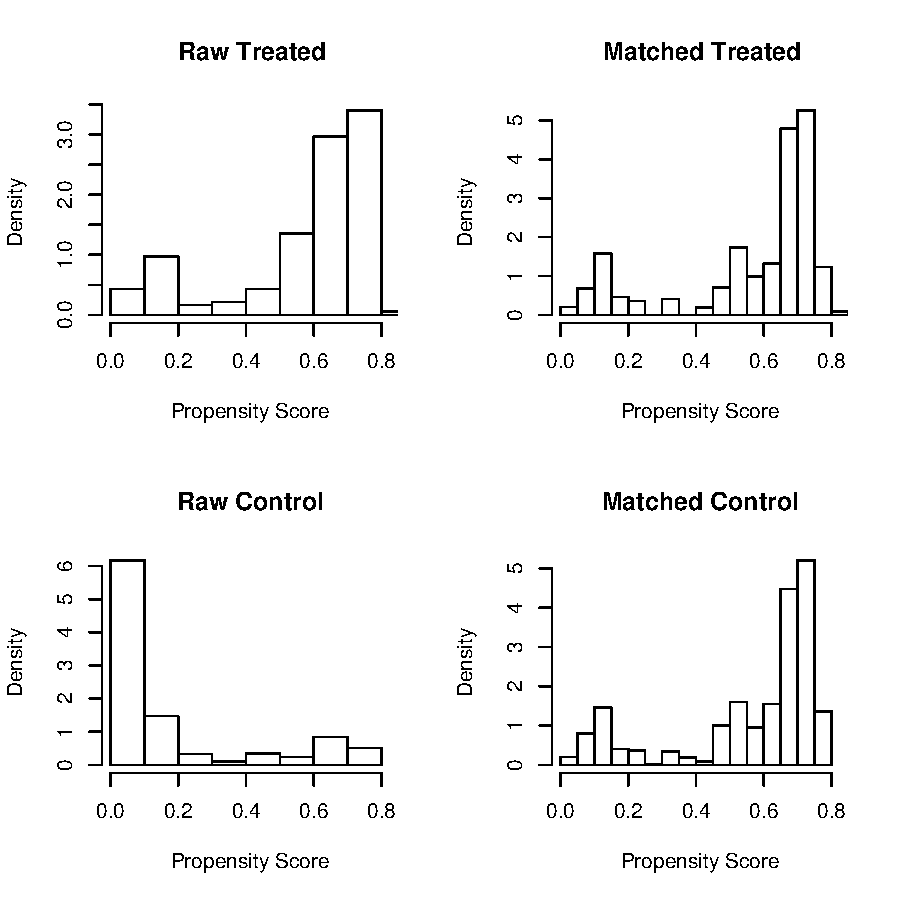
\includegraphics[height=3in]{figs/hist}
\end{center}

%%% Local Variables: 
%%% mode: latex
%%% TeX-master: "matchit"
%%% End: 

In this section, we describe our recommended approach
\citep{HoImaKin05}, which uses
\hlink{Zelig}{http://gking.harvard.edu/zelig/} to conduct parametric
causal inference after preprocessing the data through \MatchIt.  (The
resulting matched data sets can also be exported to other statistical
programs using commands such as {\tt write.csv()} and {\tt
  write.table()} for ASCII files, and {\tt write.dta} in {\tt foreign}
package for a STATA binary file.)  Zelig \citep{ImaKinLau04} is an
easy-to-use R package that implements a large variety of statistical
models, gives easily interpretable results by simulating quantities of
interest, provides numerical and graphical summaries, and is easily
extensible.  The package along with the complete documentation is
available at
\hlink{http://gking.harvard.edu/zelig/}{http://gking.harvard.edu/zelig/}.
\MatchIt\ and Zelig can be easily used together to enable estimation
of causal effects in very general settings with a variety of
statistical models.

The general syntax is as follows. First, we use \texttt{match.data()}
to create the matched data by excluding unmatched units from the
original data, and including information about the particular matching
procedure (i.e., weights, subclasses, and the distance measure).
\begin{Schunk}
\begin{Sinput}
> m.data <- match.data(m.out)
\end{Sinput}
\end{Schunk}
where {\tt m.out} is the \MatchIt\ object from {\tt matchit()} and
{\tt m.data} is the resulting matched data.  Next, we analyze the
matched data set via the following command,
\begin{Schunk}
\begin{Sinput}
> z.out <- zelig(Y ~ treat + x1 + x2, model = mymodel, data = m.data)
\end{Sinput}
\end{Schunk}
where {\tt Y} is the outcome variable, {\tt mymodel} is the selected
model, and {\tt z.out} is the output object from {\tt zelig}.

To illustrate this approach, we provide two detailed examples using
the Lalonde data. Users can run these example commands by typing {\tt
  demo(Zelig)} at the R prompt. Although we use the linear least
squares model in these examples, a wide range of other models are
available in Zelig (for the list of supported models, see
\hlink{http://gking.harvard.edu/zelig/docs/Models\_Zelig\_Can.html}{http://gking.harvard.edu/zelig/docs/Models_Zelig_Can.html}).
If you have not installed Zelig, follow the installation procedure
described at
\hlink{http://gking.harvard.edu/zelig/docs/Installation.html}{http://gking.harvard.edu/zelig/docs/Installation.html}
To load the Zelig package after installing it, type

\begin{Schunk}
\begin{Sinput}
> library(Zelig)
\end{Sinput}
\end{Schunk}

\paragraph{Examples}
\begin{enumerate}
\item We begin our first example by conducting the nearest neighbor
  matching using the estimated propensity score from the logistic
  regression
\begin{Schunk}
\begin{Sinput}
> m.out1 <- matchit(treat ~ age + educ + black + hispan + 
+     nodegree + married + re74 + re75, method = "nearest", 
+     data = lalonde)
\end{Sinput}
\end{Schunk}
Note that we skip an important step of checking balance in this
example in order to focus on the illustration of analyzing matched
data sets. We then fit the linear model to the control group
controlling for the estimated propensity score and other covariates,
\begin{Schunk}
\begin{Sinput}
> z.out1 <- zelig(re78 ~ age + educ + black + hispan + nodegree + 
+     married + re74 + re75 + distance, data = match.data(m.out1, 
+     "control"), model = "ls")
\end{Sinput}
\end{Schunk}
where the {\tt "control"} option in {\tt match.data()} extracts the
matched control units and {\tt ls} specifies linear regression. Note
that we need not include the treatment indicator in this regression.
Next, we set the covariates to the covariate values of the matched treated units
and use conditional prediction by setting the {\tt setx()} command optionsn to {\tt cond = TRUE} and {\tt
  fn = NULL} in order to impute the
counterfactual outcomes for the treated units. The {\tt sim()} command in
Zelig does the imputation.
\begin{Schunk}
\begin{Sinput}
> x.out1 <- setx(z.out1, data = match.data(m.out1, "treat"), 
+     fn = NULL, cond = TRUE)
> s.out1 <- sim(z.out1, x = x.out1)
\end{Sinput}
\end{Schunk}
Finally, we obtain a summary of the results by 
\begin{Schunk}
\begin{Sinput}
> summary(s.out1)
\end{Sinput}
\begin{Soutput}

  Model: ls 
  Number of simulations: 1000 

Mean Values of Observed Data (n = 185) 
(Intercept)         age        educ       black      hispan    nodegree 
  1.000e+00   2.582e+01   1.035e+01   8.432e-01   5.946e-02   7.081e-01 
    married        re74        re75    distance 
  1.892e-01   2.096e+03   1.532e+03   5.774e-01 

Pooled Expected Values: E(Y|X)
   mean      sd    2.5%   97.5% 
 4989.5  2304.9   684.1 10027.6 

Pooled Average Treatment Effect: Y - EV
  mean     sd   2.5%  97.5% 
1359.6  593.3  248.4 2590.4 

\end{Soutput}
\end{Schunk}
The results indicate that the estimated average treatment effect on
the treated is 
\$1359.6,
with a 95\% interval of
(\$248.4,
\$2590.4).

It is also possible to estimate the average treatment effects on both
the treated and the control groups. To do this, we fit the linear
model to the {\it treatment group} controlling for the propensity
score ({\tt distance}) and other covariates,
\begin{Schunk}
\begin{Sinput}
> z.out2 <- zelig(re78 ~ age + educ + black + hispan + nodegree + 
+     married + re74 + re75 + distance, data = match.data(m.out1, 
+     "treat"), model = "ls")
\end{Sinput}
\end{Schunk}
We then conduct the same simulation procedure in order to impute the
counterfactual outcome for the {\it control group},
\begin{Schunk}
\begin{Sinput}
> x.out2 <- setx(z.out2, data = match.data(m.out1, "control"), 
+     fn = NULL, cond = TRUE)
> s.out2 <- sim(z.out2, x = x.out2)
\end{Sinput}
\end{Schunk}
Finally, note that Zelig calculates the difference between observed
and either predicted or expected values.  This means that the
treatment effect for the control units is actually the effect of
control (observed control outcome minus the imputed outcome under
treatment from the model).  Hence, to combine treatment effects just
reverse the signs of the estimated treatment effect of controls.
\begin{Schunk}
\begin{Sinput}
> ate.all <- c(s.out1$qi$ate.ev, -s.out2$qi$ate.ev)
\end{Sinput}
\end{Schunk}
The point estimate and its standard error is given by
\begin{Schunk}
\begin{Sinput}
> mean(ate.all)
\end{Sinput}
\begin{Soutput}
[1] 1624

\end{Soutput}
\begin{Sinput}
> sd(ate.all)
\end{Sinput}
\begin{Soutput}
[1] 794.5

\end{Soutput}
\end{Schunk}
The 95\% confidence interval is given by
\begin{Schunk}
\begin{Sinput}
> quantile(ate.all, c(0.025, 0.975))
\end{Sinput}
\begin{Soutput}
  2.5%  97.5% 
 205.3 3320.5 

\end{Soutput}
\end{Schunk}
  
\item Our second example is subclassification. In this case, the
  average treatment effect estimates are obtained separately for each subclass
  as well as for the overall sample.  Estimating the
  treatment effects separately for each subclass, and then aggregating
  across subclasses, can significantly increase the robustness of the
  ultimate results since the parametric analysis within each subclass
  requires only local rather than global assumptions.

  We begin this example by conducting subclassification with four subclasses,
\begin{Schunk}
\begin{Sinput}
> m.out2 <- matchit(treat ~ age + educ + black + hispan + 
+     nodegree + married + re74 + re75, data = lalonde, method = "subclass", 
+     subclass = 4)
\end{Sinput}
\end{Schunk}
Here, we skip the important step of checking balance in order to focus
on the illustration of analyzing subclassified data sets.  Next, we
fit the linear regression within each subclass by controlling for the
estimated propensity score and past income variables within each
subclass by using the {\tt by} option in the {\tt zelig()} command. 
\begin{Schunk}
\begin{Sinput}
> z.out3 <- zelig(re78 ~ re74 + re75 + distance, data = match.data(m.out2, 
+     "control"), model = "ls", by = "subclass")
\end{Sinput}
\end{Schunk}
The same set of commands as in the first example are used to
do the imputation of the counterfactual outcomes for the treated
units.
\begin{Schunk}
\begin{Sinput}
> x.out3 <- setx(z.out3, data = match.data(m.out2, "treat"), 
+     fn = NULL, cond = TRUE)
> s.out3 <- sim(z.out3, x = x.out3)
\end{Sinput}
\end{Schunk}
Finally, to obtain the overall results, type
\begin{Schunk}
\begin{Sinput}
> summary(s.out3)
\end{Sinput}
\begin{Soutput}

  Model: ls 
  Number of simulations: 250 

Mean Values of Observed Data (n = 46) 
(Intercept)        re74        re75    distance 
     1.0000   5430.5389   2929.0394      0.2392 

Pooled Expected Values: E(Y|X)
 mean    sd  2.5% 97.5% 
 4453  5150 -4994 15742 

Pooled Average Treatment Effect: Y - EV
  mean     sd   2.5%  97.5% 
1898.2 1691.6 -793.5 5478.9 

\end{Soutput}
\end{Schunk}
The results indicate that the estimated average treatment effect on
the treated is
\$1898.2,
with a 95\% interval of
(\$-793.5,
\$5478.9).
It is also possible to get the summary result for each subclass. For
example, the following command summarizes the result for the second
subclass.
\begin{Schunk}
\begin{Sinput}
> summary(s.out3, subset = 2)
\end{Sinput}
\begin{Soutput}

Results for 1 

  Model: ls 
  Number of simulations: 250 

Mean Values of Observed Data (n = 45) 
(Intercept)        re74        re75    distance 
     1.0000   1777.4221    972.3441      0.6039 

Pooled Expected Values: E(Y|X)
 mean    sd  2.5% 97.5% 
 3631  2499 -1205  9122 

Pooled Average Treatment Effect: Y - EV
  mean     sd   2.5%  97.5% 
2854.9 1266.2  356.3 5191.7 


\end{Soutput}
\end{Schunk}
  
\end{enumerate}



%%%%%%%%%%%%%%%%%%%%%%%%%%%%%%%%%%%%%%%%%%%%%%%%%%%%%%%%%%%%%%%%%%%%%%%%%%%

\chapter{Reference Manual}
\label{chap:reference}

\section{\texttt{matchit()}: Implementation of Matching Methods}
\label{sec:matchit}
Use \texttt{matchit()} to implement a variety of matching procedures
including exact matching, nearest neighbor matching,
subclassification, optimal matching, genetic matching, and full
matching.  The output of {\tt matchit()} can be analyzed via any
standard R package, by exporting the data for use in another program,
or most simply via \hlink{Zelig}{http://gking.harvard.edu/zelig} in R.

\subsubsection{Syntax}
\begin{verbatim}
> m.out <- matchit(formula, data, method = "nearest", verbose = FALSE, ...)
\end{verbatim}

\subsubsection{Arguments}

\paragraph{Arguments for All Matching Methods}

\begin{itemize}

\item \texttt{formula}: formula used to calculate the distance measure
  for matching.  It takes the usual syntax of R formulas, {\tt treat
    \~\ x1 + x2}, where {\tt treat} is a binary treatment indicator,
  and {\tt x1} and {\tt x2} are the pre-treatment covariates. Both the
  treatment indicator and pre-treatment covariates must be contained
  in the same data frame, which is specified as {\tt data} (see
  below).  All of the usual R syntax for formulas work here. For
  example, {\tt x1:x2} represents the first order interaction term
  between {\tt x1} and {\tt x2}, and {\tt I(x1 \^\ 2)} represents the
  square term of {\tt x1}. See {\tt help(formula)} for details.
  
\item \texttt{data}: the data frame containing the variables called in
  {\tt formula}.  
  
\item \texttt{method}: the matching method (DEFAULT =
  \texttt{"nearest"}, nearest neighbor matching).  Currently,
  \texttt{"exact"} (exact matching), \texttt{"full"} (full matching),
  \texttt{"nearest"} (nearest neighbor matching), \texttt{"optimal"}
  (optimal matching), \texttt{"subclass"} (subclassification), and
  \texttt{"genetic"} (genetic matching) are available. Note that
  within each of these matching methods, \MatchIt\ offers a variety of
  options. See below for more details.
  
\item \texttt{verbose}: a logical value indicating whether to print
  the status of the matching algorithm (DEFAULT = \texttt{FALSE}).
\end{itemize}


\paragraph{Additional Arguments for Specification of
  Distance Measures}
\label{subsubsec:inputs-all}

The following arguments specify distance measures that are used for
matching methods. These arguments apply to all matching methods {\it
  except exact matching}.

\begin{itemize}
  
\item \texttt{distance}: the method used to estimate the distance
  measure (DEFAULT = {\tt "logit"}, logistic regression).  Before
  using any of these techniques, it is best to understand the
  theoretical groundings of these techniques and to evaluate the
  results.  Most of these methods (such as logistic or probit
  regression) estimate the propensity score, defined as the
  probability of receiving treatment, conditional on the covariates.
  Available methods include:
  \begin{itemize}
  \item {\tt "mahalanobis"}: the Mahalanobis distance measure.
  \item binomial generalized linear models with one of the following
    link functions:
    \begin{itemize}
    \item \texttt{"logit"}: logistic link 
    \item {\tt "linear.logit"}: logistic link with linear propensity
      score)\footnote{The linear propensity scores are obtained by
        transforming back onto a linear scale.}
    \item \texttt{"probit"}: probit link
    \item {\tt "linear.probit"}: probit link with linear propensity
      score
    \item {\tt "cloglog"}: complementary log-log link
    \item {\tt "linear.cloglog"}: complementary log-log link with linear
      propensity score
    \item {\tt "log"}: log link
    \item {\tt "linear.log"}: log link with linear propensity score
    \item {\tt "cauchit"} Cauchy CDF link
    \item {\tt "linear.cauchit"} Cauchy CDF link with linear propensity
      score
    \end{itemize}
  \item Choose one of the following generalized additive models (see
    {\tt help(gam)} for more options).
    \begin{itemize}
    \item \texttt{"GAMlogit"}: logistic link
    \item {\tt "GAMlinear.logit"}: logistic link with linear propensity
      score
    \item \texttt{"GAMprobit"}: probit link
    \item {\tt "GAMlinear.probit"}: probit link with linear propensity
      score
    \item {\tt "GAMcloglog"}: complementary log-log link 
    \item {\tt "GAMlinear.cloglog"}: complementary log-log link with
      linear propensity score
    \item {\tt "GAMlog"}: log link
    \item {\tt "GAMlinear.log"}: log link with linear propensity score,
    \item {\tt "GAMcauchit"}: Cauchy CDF link
    \item {\tt "GAMlinear.cauchit"}: Cauchy CDF link with linear
      propensity score
\end{itemize} 
\item \texttt{"nnet"}: neural network model.  See {\tt help(nnet)} for
  more options.
\item \texttt{"rpart"}: classification trees.  See {\tt help(rpart)}
  for more options.
  \end{itemize}
  
\item \texttt{distance.options}: optional arguments for estimating the
  distance measure. The input to this argument should be a list.  For
  example, if the distance measure is estimated with a logistic
  regression, users can increase the maximum IWLS iterations by
  \texttt{distance.options = list(maxit = 5000)}.  Find additional
  options for general linear models using {\tt help(glm)} or {\tt
    help(family)}, for general additive models using {\tt help(gam)},
  for neutral network models {\tt help(nnet)}, and for classification
  trees {\tt help(rpart)}.
  
\item \texttt{discard}: specifies whether to discard units that fall
  outside some measure of support of the distance measure (DEFAULT =
  \texttt{"none"}, discard no units).  Discarding units may change the
  quantity of interest being estimated. Enter a logical vector
  indicating which unit should be discarded or choose from the
  following options:
  \begin{itemize}
  \item \texttt{"none"}: no units will be discarded before matching.
    Use this option when the units to be matched are substantially
    similar, such as in the case of matching treatment and control
    units from a field experiment that was close to (but not fully)
    randomized (e.g., \citealt{Imai05}), when caliper matching will
    restrict the donor pool, or when you do not wish to change the
    quantity of interest and the parametric methods to be used
    post-matching can be trusted to extrapolate.
  \item \texttt{"hull.both"}: all units that are not within the convex
    hull will be discarded.  We recommend that this option be used
    with observational data sets.
  \item \texttt{"both"}: all units (treated and control) that are
    outside the support of the distance measure will be discarded.
  \item \texttt{"hull.control"}: only control units that are not
    within the convex hull of the treated units will be discarded.  
  \item \texttt{"control"}: only control units outside the support of
    the distance measure of the treated units will be discarded.  Use
    this option when the average treatment effect on the treated is of
    most interest and when you are unwilling to discard
    non-overlapping treatment units (which would change the quantity
    of interest).
  \item \texttt{"hull.treat"}: only treated units that are not within
    the convex hull of the control units will be discarded. 
  \item \texttt{"treat"}: only treated units outside the support of
    the distance measure of the control units will be discarded.  Use
    this option when the average treatment effect on the control units
    is of most interest and when unwilling to discard control units.
  \end{itemize}
  
\item \texttt{reestimate}: If {\tt FALSE} (DEFAULT), the model for the
  distance measure will not be re-estimated after units are discarded.
  The input must be a logical value.  Re-estimation may be desirable
  for efficiency reasons, especially if many units were discarded and
  so the post-discard samples are quite different from the original
  samples.
  
\end{itemize}

\paragraph{Additional Arguments for Subclassification}
\label{subsubsec:inputs-subclass}

\begin{itemize}
\item \texttt{sub.by}: criteria for subclassification.  Choose from:
  \texttt{"treat"} (DEFAULT), the number of treatment units;
  \texttt{"control"}, the number of control units; or \texttt{"all"},
  the total number of units.
\item \texttt{subclass}: either a scalar specifying the number of
  subclasses, or a vector of probabilities bounded between 0 and 1,
  which create quantiles of the distance measure using the units in
  the group specified by \texttt{sub.by} (DEFAULT = \texttt{subclass =
    6}).
\end{itemize}

\paragraph{Additional Arguments for Nearest Neighbor Matching}
\label{subsubsec:inputs-nearest}

\begin{itemize}
\item \texttt{m.order}: the order in which to match treatment units
  with control units.
  \begin{itemize}
  \item {\tt "largest"} (DEFAULT): matches from the largest value of
    the distance measure to the smallest.
  \item {\tt "smallest"}: matches from the smallest value of the
    distance measure to the largest.
  \item {\tt "random"}: matches in random order.
  \end{itemize}
\item \texttt{replace}: logical value indicating whether each control
  unit can be matched to more than one treated unit (DEFAULT = {\tt
    replace = FALSE}, each control unit is used at most once -- i.e.,
  sampling without replacement). For matching with replacement, use
  \texttt{replace = TRUE}.
\item \texttt{ratio}: the number of control units to match to each
  treated unit (DEFAULT = {\tt 1}).  If matching is done without
  replacement and there are fewer control units than {\tt ratio} times
  the number of eligible treated units (i.e., there are not enough
  control units for the specified method), then the higher ratios will
  have \texttt{NA} in place of the matching unit number in
  \texttt{match.matrix}.
\item \texttt{exact}: variables on which to perform exact matching
  within the nearest neighbor matching (DEFAULT = {\tt NULL}, no exact
  matching).  If \texttt{exact} is specified, only matches that
  exactly match on the covariates in \texttt{exact} will be allowed.
  Within the matches that match on the variables in \texttt{exact},
  the match with the closest distance measure will be chosen.
  \texttt{exact} should be entered as a vector of variable names
  (e.g., \texttt{exact = c("X1", "X2")}).
\item \texttt{caliper}: the number of standard deviations of the
  distance measure within which to draw control units (DEFAULT = {\tt
    0}, no caliper matching).  If a caliper is specified, a control
  unit within the caliper for a treated unit is randomly selected as
  the match for that treated unit.  If \texttt{caliper != 0}, there
  are two additional options:
  \begin{itemize} 
  \item \texttt{calclosest}: whether to take the nearest available
    match if no matches are available within the \texttt{caliper}
    (DEFAULT = {\tt FALSE}).
  \item \texttt{mahvars}: variables on which to perform
    Mahalanobis-metric matching within each caliper (DEFAULT = {\tt
      NULL}).  Variables should be entered as a vector of variable
    names (e.g., \texttt{mahvars = c("X1", "X2")}).  If
    \texttt{mahvars} is specified without \texttt{caliper}, the
    caliper is set to 0.25.
  \end{itemize}
\item \texttt{subclass} and \texttt{sub.by}: See the options for
  subclassification for more details on these options.  If a
  \texttt{subclass} is specified within \texttt{method = "nearest"},
  the matched units will be placed into subclasses after the nearest
  neighbor matching is completed.
\end{itemize}

\paragraph{Additional Arguments for Optimal Matching}
\label{subsubsec:inputs-optimal}

\begin{itemize}
\item {\tt ratio}: the number of control units to be matched to each
  treatment unit (DEFAULT = {\tt 1}).
\item {\tt ...}: additional inputs that can be passed to the {\tt
    fullmatch()} function in the {\tt optmatch} package. See {\tt
    help(fullmatch)} or
  \hlink{http://www.stat.lsa.umich.edu/\~{}bbh/optmatch.html}{http://www.stat.lsa.umich.edu/\~bbh/optmatch.html}
  for details.
\end{itemize}

\paragraph{Additional Arguments for Full Matching}
\label{subsubsec:inputs-full}

\begin{itemize}
\item {\tt ...}: additional inputs that can be passed to the {\tt
    fullmatch()} function in the {\tt optmatch} package. See {\tt
    help(fullmatch)} or
  \hlink{http://www.stat.lsa.umich.edu/\~{}bbh/optmatch.html}{http://www.stat.lsa.umich.edu/\~bbh/optmatch.html}
  for details.
\end{itemize}

\paragraph{Additional Arguments for Genetic Matching}
\label{subsubsec:inputs-genetic}

The available options are listed below.
\begin{itemize}
\item {\tt ratio}: the number of control units to be matched to each
  treatment unit (DEFAULT = {\tt 1}).
\item {\tt ...}: additional minor inputs that can be passed to the
  {\tt GenMatch()} function in the {\tt Matching} package. See {\tt
    help(GenMatch)} or
  \hlink{http://sekhon.polisci.berkeley.edu/library/Matching/html/GenMatch.html}{http://sekhon.polisci.berkeley.edu/library/Matching/html/GenMatch.html}
  for details.
\end{itemize}

\subsubsection{Output Values}
\label{sec:outputs}

Regardless of the type of matching performed, the \texttt{matchit}
output object contains the following elements:\footnote{When
  inapplicable or unnecessary, these elements may equal {\tt NULL}.
  For example, when exact matching, {\tt match.matrix = NULL}.}

\begin{itemize}
\item \texttt{call}: the original {\tt matchit()} call.
  
\item \texttt{formula}: the formula used to specify the model for
  estimating the distance measure.
  
\item \texttt{model}: the output of the model used to estimate
  the distance measure.  \texttt{summary(m.out\$model)} will give the
  summary of the model where \texttt{m.out} is the output object from
  \texttt{matchit()}.
  
\item \texttt{match.matrix}: an $n_1 \times$ \texttt{ratio} matrix
  where:
  \begin{itemize}
  \item the row names represent the names of the treatment units
    (which match the row names of the data frame specified in
    \texttt{data}).
  \item each column stores the name(s) of the control unit(s) matched
    to the treatment unit of that row. For example, when the
    \texttt{ratio} input for nearest neighbor or optimal matching is
    specified as 3, the three columns of \texttt{match.matrix}
    represent the three control units matched to one treatment unit).
  \item \texttt{NA} indicates that the treatment unit was not matched.
  \end{itemize}
  
\item \texttt{discarded}: a vector of length $n$ that displays whether
  the units were ineligible for matching due to common support
  restrictions.  It equals \texttt{TRUE} if unit $i$ was discarded,
  and it is set to \texttt{FALSE} otherwise.
  
\item \texttt{distance}: a vector of length $n$ with the estimated
  distance measure for each unit.
  
\item \texttt{weights}: a vector of length $n$ with the weights
  assigned to each unit in the matching process.  Unmatched units have
  weights equal to $0$. Matched treated units have weight $1$.  Each
  matched control unit has weight proportional to the number of
  treatment units to which it was matched, and the sum of the control
  weights is equal to the number of uniquely matched control units.
 
\item \texttt{subclass}: the subclass index in an ordinal scale from 1
  to the total number of subclasses as specified in \texttt{subclass}
  (or the total number of subclasses from full or exact matching).
  Unmatched units have \texttt{NA}.
  
\item \texttt{q.cut}: the subclass cut-points that classify the
  distance measure.
  
\item \texttt{treat}: the treatment indicator from \texttt{data} (the
  left-hand side of \texttt{formula}).
 
\item \texttt{X}: the covariates used for estimating the distance
  measure (the right-hand side of \texttt{formula}).  When applicable,
  \texttt{X} is augmented by covariates contained in \texttt{mahvars}
  and \texttt{exact}.
\end{itemize}

\subsubsection{Contributors}

If you use \MatchIt, please cite
\begin{verse}
\bibentry{HoImaKin05}
and 
\bibentry{HoImaKin05b}
\end{verse}

The {\tt convex.hull} discard option is implemented via the {\tt
  WhatIf} package.  If you use this option, please cite
\begin{verse}
\bibentry{StoKinZen05} 
and either
\bibentry{KinZen06a}
or
\bibentry{KinZen06b}
\end{verse} 

Generalized linear distance measures are implemented via the {\tt
stats} package.  If you use this distance measure, please cite 
\begin{verse}
\bibentry{VenRip02}
\end{verse}

Generalized additive distance measures are implemented via the {\tt
  mcgv} package.  If you use this distance measure, please cite
\begin{verse}
\bibentry{HasTib90}
\end{verse}  

The neural network distance measure is implemented via the {\tt nnet}
package.  If you use this distance measure, please cite
\begin{verse}
\bibentry{Ripley96}
\end{verse}

The classification trees distance measure is implemented via the {\tt
  rpart} package.  If you use this distance measure, please cite
\begin{verse}
\bibentry{BreFriOls84}
\end{verse}  

Full and optimal matching are implemented via the {\tt optmatch}
package by Ben Hansen. If you use either of these methods, please cite
\begin{verse}
\bibentry{Hansen04}
\end{verse} 

Genetic matching is implemented via the {\tt Matching} package by
Jasjeet Sekhon.  If you use this method, please cite
\begin{verse}
\bibentry{DiaSek05}
\end{verse}

%%% Local Variables: 
%%% mode: latex
%%% TeX-master: "matchit"
%%% End: 

\section{\texttt{summary()}: Numerical Summaries of Balance}

\subsection{Description}
The \texttt{summary()} command returns numerical summaries of balance
diagnostics.

\subsection{Syntax}
\begin{verbatim}
summary(object, interactions = FALSE, addlvariables = NULL, ...)
\end{verbatim}

\subsection{Arguments}

\begin{itemize}
\item \texttt{object}: the output from {\tt matchit()}.
\item \texttt{interactions}: an option to calculate summary
  statistics in \texttt{sum.all} and \texttt{sum.matched} for all
  covariates, their squares, and two-way interactions when
  \texttt{interactions = TRUE} and only the covariates themselves when
  \texttt{interactions = FALSE} (default).
\item \texttt{addlvariables}: additional variables on which to
  calculate the diagnostic statistics (in addition to the variables
  included in the matching procedure) (default = NULL).
  \texttt{addlvariables}: a data frame containing additional variables
  whose balance is examined. The data should come with the same number
  of units and units in the same order as in the data set used for
  {\tt matchit()}.
\end{itemize}

\subsection{Output Values}

The output from the \texttt{summary()} command includes the following
elements, when applicable:
\begin{itemize}
\item The original assignment model call.
\item \texttt{sum.all}: a data frame that contains variable names and
  interactions down the row names, and summary statistics on \emph{all
    observations} in each of the columns.  The columns in
  \texttt{sum.all} contain \footnote{The output for full matching is
    slightly different from that described here; see Section
    \ref{subsubsec:full} for details.}:
  \begin{itemize}
  \item means of all covariates $X$ for treated and control units,
    where \texttt{Means Treated}$= \mu_{X|T=1} = \frac{1}{n_1}
    \sum_{T=1} X_i$ and \texttt{Means Control}$= \mu_{X|T=0} =
    \frac{1}{n_0} \sum_{T=0} X_i$,
  \item standard deviation in the treated group for all covariates $X$,  
        $$\quad s_{x|T=1} = \sqrt{\frac{\sum_{i \in \{i: T_i=1\}}
        (X_i - \mu_{X|T=1}}{n_1-1})^2 }.$$
  \item summary statistics from a Q-Q plot, which compares treated and
    control covariate distributions, where \texttt{QQ Med}, \texttt{QQ
      Mean}, and \texttt{QQ Max} indicate the median, mean, and
    maximum orthogonal deviations from the 45 degree line of a Q-Q
    plot.
  \item standardized bias statistics, $${\rm Std.
      Bias}=\frac{\mu_{X|T=1} - \mu_{X|T=0}}{s_{x|T=1}}.$$
  \end{itemize}
  
\item \texttt{sum.matched}: a data frame which contains variable names
  down the row names, and summary statistics on only the \emph{matched
    observations} in each of the columns.  Specifically, the columns
  in \texttt{sum.matched} contain the following elements\footnote{The
    values output for full matching are slightly different from that
    described here; see Section \ref{subsubsec:full} for details}:
  \begin{itemize}
  \item weighted means for matched treatment units of all covariates
    $X$ and their interactions, where \texttt{Means Treated}$=
    \mu_{wX|T=1} = \frac{1}{n_1} \sum_{T=1} w_iX_i$ and \texttt{Means
      Control}$=\mu_{wX|T=0} = \frac{1}{n_0} \sum_{T=0} w_iX_i$,
  \item weighted standard deviations in the matched treated group for
    all covariates $X$, where \texttt{SD} $= s_{wX} =
    \sqrt{\frac{1}{n} \sum_{i} (w_iX_i - \overline{X}^*)^2}$, where
    $\overline{X}^*$ is the weighted mean of $X$ in the matched
    treated group, and
  \item standardized bias statistics \texttt{Std.
      Bias}$=\frac{\mu_{wX|T=1} - \mu_{wX|T=0}}{s_{x|T=1}}$.
  \end{itemize}
  where $w$ represents the vector of \texttt{weights}.
  
\item \texttt{reduction}: the percent bias reduction achieved in each
  of the balance measures in \texttt{sum.all} and
  \texttt{sum.matched}, defined as $100(|a|-|b|)/|a|$, where $a$ was
  the value of the balance measure before matching and $b$ is the
  value of the balance measure after matching.  Because the difference
  in means and the standardized bias differ only by a constant (the
  standard deviation in the full treated group), the percent reduction
  in bias is the same for these two measures, and thus is only printed
  out once.
  
\item \texttt{nn}: the sample sizes in the full and matched samples
  and the number of discarded units, by treatment and control.
  
\item \texttt{q.table}: an array that contains the same information
  as \texttt{sum.matched} by subclass.
  
\item \texttt{qn}: the sample sizes in the full and matched
  samples and the number of discarded units, by subclass and by
  treatment and control.
\item \texttt{match.matrix}: the same object is contained in the
  output of {\tt matchit()}.
\end{itemize}

%%% Local Variables: 
%%% mode: latex
%%% TeX-master: "matchit"
%%% End: 

\section{\texttt{plot()}: Graphical Summaries of Balance}

The \texttt{plot()} command allows you to check the distributions of
covariates in the assignment model, squares, and interactions, and
within each subclasses if specified.  

\subsubsection{Syntax}

\begin{verbatim}
> plot(m.out, discrete.cutoff = 5, type = "QQ", 
       numdraws = 5000, interactive = TRUE, which.xs = NULL, ...)
\end{verbatim}

\subsubsection{Arguments}

\begin{itemize}
\item {\tt type}: type of output graph. \texttt{type = "QQ"}
  (default) outputs empirical quantile-quantile plots of each
  covariate to check balance of marginal distributions. Alternatively,
  \texttt{type = "jitter"} outputs jitter plots of the propensity
  score for treated and control units.
  
\item {\tt discrete.cutoff}: For quantile-quantile plots, discrete
  covariates that take 5 or fewer values are jittered for visibility.
  This may be changed by setting this argument to any other positive
  integer.
  
\item {\tt interactive}: If \texttt{TRUE} (default), users can
  identify individual units by clicking on the graph with the left
  mouse button, and (when applicable) choose subclasses to plot.
  
\item {\tt which.xs}: Specifies particular covariate names in a
  character vector to plot only a subset of the covariates.

\item {\tt subclass}: If \texttt{interactive = FALSE}, users can
  specify which subclass to plot. 

\end{itemize}

\subsubsection{Output Values}

\begin{itemize}
\item Empirical quantile-quantile plot: This graph plots covariate
  values that fall in (approximately) the same quantile of treated and
  control distributions.  Control unit quantile values are plotted on
  the x-axis, and treated unit quantile values are plotted on the
  y-axis.  If values fall below the 45 degree line, control units
  generally take lower values of the covariate.  Data points that fall
  exactly on the 45 degree line indicate that the marginal
  distributions are identical.
  
\item Jitter plots: This graph plots jittered estimated propensity
  scores of treated and control units.  Dark diamonds indicate matched
  units and grey diamonds indicate unmatched or discarded units.  The
  area of the diamond is proportional to the weights. Vertical lines
  are plotted if subclassification is used.

\end{itemize}


%%% Local Variables: 
%%% mode: latex
%%% TeX-master: "matchit"
%%% End: 


\section{\texttt{match.data()}: Extracting the Matched Data Set}
\label{sec:match.data}

\subsection{Usage}

To extract the matched data set for subsequent analyses from the
output object (see Section~\ref{sec:analysis}), we provide the
function {\tt match.data()}.  This is used as follows:

\begin{verbatim}
> m.data <- match.data(object, group = "all", distance = "distance", 
                       weights = "weights", subclass = "subclass")
\end{verbatim}

The output of the function {\tt match.data()} is the original data
frame where additional information about matching (i.e., distance
measure as well as resulting weights and subclasses) is added,
restricted to units that were matched.

\subsection{Arguments}

{\tt match.data()} takes the following inputs:
\begin{enumerate}
\item {\tt object} is the output object from {\tt matchit()}. This is
  a required input.
\item {\tt group} specifies for which matched group the user wants to
  extract the data. Available options are {\tt "all"} (all matched
  units), {\tt "treat"} (matched units in the treatment group), and
  {\tt "control"} (matched units in the control group). The default is
  {\tt "all"}.
\item {\tt distance} specifies the variable name used to store the
  distance measure. The default is {\tt "distance"}.
\item {\tt weights} specifies the variable name used to store the
  resulting weights from matching. The default is {\tt "weights"}. See
  Section~\ref{subsec:weights} for more details on the weights.
\item {\tt subclass} specifies the variable name used to store the
  subclass indicator. The default is {\tt "subclass"}.
\end{enumerate}

\subsection{Examples}

Here, we present examples for using {\tt match.data()}. Users can run
these commands by typing {\tt demo(match.data)} at the R
prompt. First, we load the Lalonde data,

\begin{verbatim}
> data(lalonde)
\end{verbatim}

The next line performs nearest neighbor matching based on the
estimated propensity score from the logistic regression,

\begin{verbatim}
> m.out1 <- matchit(treat ~ re74 + re75 + age + educ, data = lalonde, 
+     method = "nearest", distance = "logit")
\end{verbatim}

To obtain matched data, type the following command, 

\begin{verbatim}
> m.data1 <- match.data(m.out1)
\end{verbatim}

It is easy to summarize the resulting matched data,

\begin{verbatim}
> summary(m.data1)
\end{verbatim}

To obtain matched data for the treatment or control group, specify the option
{\tt group} as follows,

\begin{verbatim}
> m.data2 <- match.data(m.out1, group = "treat")
> summary(m.data2)
> m.data3 <- match.data(m.out1, group = "control")
> summary(m.data3)
\end{verbatim}

We can also use the function to return unmatched data:

\begin{verbatim}
> unmatched.data <- lalonde[!row.names(lalonde)%in%row.names(match.data(m.out1)),]
\end{verbatim}

We can also specify different names for the subclass indicator, the
weight variable, and the estimated distance measure. The following
example first does a subclassification method, obtains the
matched data with specified names for those three variables, and then
print out the names of all variables in the resulting matched data.

\begin{verbatim}
> m.out2 <- matchit(treat ~ re74 + re75 + age + educ, data = lalonde, 
+     method = "subclass")
> m.data4 <- match.data(m.out2, subclass = "block", weights = "w", 
+     distance = "pscore")
> names(m.data4)
\end{verbatim}

%%% Local Variables: 
%%% mode: latex
%%% TeX-master: "matchit"
%%% End: 

\chapter{Frequently Asked Questions}

\section{How do I Cite this Work?}

If you use \MatchIt, please cite\nocite{HoImaKin07,HoImaKin07a}
\begin{verse}
  Daniel Ho; Kosuke Imai; Gary King; and Elizabeth Stuart (2007),
  ``Matching as Nonparametric Preprocessing for Reducing Model
  Dependence in Parametric Causal Inference,'' \emph{Political
    Analysis} 15(3): 199-236,
  \url{http://gking.harvard.edu/files/abs/matchp-abs.shtml}.

and 

Daniel Ho; Kosuke Imai; Gary King; and Elizabeth Stuart (2007b)
``Matchit: Nonparametric Preprocessing for Parametric Causal
Inference,'' \emph{Journal of Statistical Software},
\url{http://gking.harvard.edu/matchit/}.
\end{verse}

In addition, the {\tt convex.hull} discard option is implemented via
the {\tt WhatIf} package \citep{KinZen06,KinZen07,StoKinZen05}.
Generalized linear distance measures are implemented via the {\tt
  stats} package \citep{VenRip02}.  Generalized additive distance
measures are implemented via the {\tt mcgv} package \citep{HasTib90}.
The neural network distance measure is implemented via the {\tt nnet}
package \citep{Ripley96}.  The classification trees distance measure
is implemented via the {\tt rpart} package \citep{BreFriOls84}.  Full
and optimal matching are implemented via the {\tt optmatch} package
\citep{Hansen04}.  Genetic matching is implemented via the {\tt
  Matching} package \citep{DiaSek05}.  Coarsened exact matching is
implemented via the \texttt{cem} package
\citep{IacKinPor08,IacKinPor08b}.

\section{What if My datasets Are Big and Are Taking Up
  Too Much Memory?}

{\tt matchit()} does not save the data set in its output object, but
it does save a matrix of the covariates.  {\tt match.data()} will
create a matched data set. One can eliminate the original data set to
save memory in R by {\tt rm(name)}, where {\tt name} is the name of
the data set, after calling {\tt match.data()}.

%\section{Can I use a Difference-in-Difference Estimator for Matched
%  Data?}
%
%A difference-in-differences (DID) analysis can be easily conducted
%with \MatchIt.  If we were interested in the DID matching estimate in
%the Lalonde data, we could simply include {\texttt re75} as a
%covariate in the preprocessing step.  Then the analysis can be
%performed on the change in income from 1975 to 1978: {\tt re78}-{\tt
%  re75}.  Time-varying covariates (of which none exist in the Lalonde
%data) should of course also be differenced for the DID estimator.
%** we should show how to do this with zelig

\section{How Exactly are the Weights Created?}
\label{subsec:weights}

Each type of matching method can be thought of as creating groups of
units with at least one treated unit and at least one control unit in
each.  In exact matching, subclassification, or full matching, these
groups are the subclasses formed, and the number of treated and
control units will vary quite a bit across subclasses.  In nearest
neighbor or optimal matching, the groups are the pairs (or sets) of
treated and control units matched.  In 1:1 nearest neighbor matching
there will be one treated unit and one control unit in each group.  In
2:1 nearest neighbor matching there will be one treated unit and two
control units in each group.  Unmatched units receive a weight of 0.
All matched treated units receive a weight of 1.  These weights are constructed
to estimate the average treatment effect on the treated, with the control group
essentially weighted to look like the treated group.

The weights for matched control units are formed as follows:
\begin{enumerate}
\item Within each group, each control unit is given a preliminary
  weight of $n_{ti}/n_{ci}$, where $n_{ti}$ and $n_{ci}$ are the
  number of treated and control units in group $i$, respectively.
\item If matching is done with replacement, each control unit's weight
  is added up across the groups in which it was matched.
\item The control group weights are scaled to sum to the number of
  uniquely matched control units.
\end{enumerate}

With subclassification, when the analysis is done separately within
each subclass and then aggregated up across the subclasses, these
weights will generally not be used, but they may be used for full
matching or nearest neighbor matching if the number of control units
matched to each treated unit varies.



\section{How Do I Create Observation Names?}
\label{rnames}

Since the diagnostics often make use of the observation names of the
data frame, you may find it helpful to specify observation names for
the data input.  Use the \texttt{row.names} command to achieve this.
For example, to assign the names ``Dan'', ``Kosuke'', ``Liz'' and
``Gary'' to a data frame with the first four observations in the
Lalonde data, type:


\begin{verbatim}
> test <- lalonde[1:4, ]
> row.names(test) <- c("Dan", "Kosuke", "Liz", "Gary")
> print(test)
       age educ black hisp married nodegr re74 re75  re78 u74 u75 treat
Dan     37   11     1    0       1      1    0    0  9930   1   1     1
Kosuke  22    9     0    1       0      1    0    0  3596   1   1     1
Liz     30   12     1    0       0      0    0    0 24910   1   1     1
Gary    27   11     1    0       0      1    0    0  7506   1   1     1
\end{verbatim}

\section{How Can I See Outcomes of Matched Pairs?}

To obtain outcomes of matched pairs, recall that the original dataset has unique row names corresponding to each of
the observations.  The row names of \texttt{match.matrix} correspond to the names of the treated, and each
of the cells corresponds to a name of matched controls.  So to obtain matched outcomes, you can use:

\begin{verbatim}
cbind(lalonde[row.names(foo$match.matrix),"re78"], lalonde[foo$match.matrix,"re78"])
\end{verbatim}

\section{How Do I Ensure Replicability As \MatchIt\ Versions Develop?}
\label{subsec:vercontrol}

As the literature on matching techniques is rapidly evolving,
\MatchIt\ will strive to incorporate new developments. \MatchIt\ is
thereby an evolving program.  Users may be concerned that analysis
written in a particular version may not be compatible with newer
versions of the program.  The primary way to ensure that replication
archives remain valid is to record the version of \MatchIt\ that was
used in the analysis.  Our website maintains binaries of all public
release versions, so that researchers can replicate results exactly
with the appropriate version (for Unix-based platforms, see
\hlink{http://gking.harvard.edu/src/contrib/}{http://gking.harvard.edu/src/contrib/};
for windows, see
\hlink{http://gking.harvard.edu/bin/windows/contrib/}{http://gking.harvard.edu/bin/windows/contrib/}).

In addition, users may find it helpful to install packages with
version control, using the {\tt installWithVers} command with {\tt
install.packages}.  So for example, in the windows R console, users
may download the appropriate version from our website and install the
package with version control by:

\begin{verbatim}
install.packages(choose.files('',filters=Filters[c('zip','All'),]),
                 .libPaths()[1],installWithVers=T,CRAN=NULL)
\end{verbatim}

{\tt R CMD INSTALL} similarly permits users to specify this version
using the \\ {\tt --with-package-versions} option.  After having
specified version control, different versions of the program may be
called as necessary.  Similar advice may also be appropriate for
version control for R more generally.

\section{How Do I Use My Own Distance Measure with \MatchIt\,?}

A vector of your own distance measure can be used by specifying it as
the input for {\tt distance} option in {\tt matchit()}.

\section{What Do I Do about Missing Data?}

\MatchIt\ requires complete data sets, with no missing values (other
than potential outcomes of course).  If there are missing values in
the data set, imputation techniques should be used first to fill in
(``impute'') the missing values (both covariates and outcomes), or the
analysis should be done using only complete cases (which we do not in
general recommend).  For imputation software, see Amelia at
(\hlink{http://gking.harvard.edu/stats.shtml}{http://gking.harvard.edu/stats.shtml})
or other programs at
\hlink{http://www.multiple-imputation.com}{http://www.multiple-imputation.com}.
For more information on missing data and imputation methods, see
\cite{KinHonJos01}.

\section{Why Preprocessing?}

The purpose of matching is to approximate an experimental template,
where the matching procedure approximates blocking prior to random
treatment assignment in order to balance covariates between treatment
and control groups.  Separation of the estimation procedure into two
steps simulates the research design of an experiment, where no
information on outcomes is known at the point of experimental design
and randomization.  The separation of the balancing process in
\MatchIt\ from the analysis process afterward helps keep clear the
goal of balancing control and treatment groups and makes it less
likely that the user will inadvertently cook the books in his or her
favor.


%%% Local Variables: 
%%% mode: latex
%%% TeX-master: t
%%% End: 


%%%%%%%%%%%%%%%%%%%%%%%%%%%%%%%%%%%%%%%%%%%%%%%%%%%%%%%%%%%%%%%%%%%%%%%%%

%%%%%%%%%%%%%%%%%%%%%%%%%%%%%%%%%%%%%%%%%%%%%%%%%%%%%%%%%%%%%%%%%%%%%%%%%


\chapter{What's New?}

\begin{itemize}
\item \textbf{2.4-20} (October 24, 2011): bug fix for GAM models (thanks to Felix Thoemmes)
\item \textbf{2.4-18} (April 26, 2011): JSS version, no change in code.
\item \textbf{2.4-17} (April 2, 2011): a minor documentation fix.
\item \textbf{2.4-16} (January 8, 2011): a bug fix for user defined distance.
\item \textbf{2.4-15} (December 11, 2010): a bug fix in the
  mahalanobis matching.
\item \textbf{2.4-14} (August 12, 2010): a bug fix in {\tt
    match.data()} so that it can be called within a function (thanks
  to Ajay Shah, George Baah, and Ben Dominique); \MatchIt now does not
  specify digits for printing (thanks to Chris Hane); A summary table
  of matched data is now stored in the output (thanks to George Baah)
\item \textbf{2.4-11} (June 25, 2009): More flexible inputs in
  plotting.
\item \textbf{2.4-10} (February 2, 2009): Minor documentation fixes
\item \textbf{2.4-8,2.4-9} (January 29, 2009): Minor documentation fixes
\item \textbf{2.4-7} (August 4, 2008): Fixed minor bug in subclassification 
(thanks to Ben Domingue)
\item \textbf{2.4-6} (July 21, 2008): Improved summary object for
  exact matching (thanks to Andrew Stokes)
\item \textbf{2.4-5} (July 20, 2008): Fixed a minor bug.
\item \textbf{2.4-4} (July 18, 2008): Fixed another bug with regard to the discard option (thanks to Ben Dominique).
\item \textbf{2.4-3} (July 18, 2008): Fixed a bug in full matching
  regarding the discard option (thanks to Ben Dominique). Some updates
  of documentation regarding coarsened exact matching (2.4-1 and
  2.4-2).
\item \textbf{2.4} (June 12, 2008): Included coarsened exact matching;
  documentation bug fixes (thanks to Will Lowe)
\item \textbf{2.3-1} (October 11, 2007): Stable release for R
  2.6. Documentation improved. Some minor bug fixes and improvements.
\item \textbf{2.2-14} (September 2, 2007): Stable release for R 2.5.
  Documentation improved for full matching. (Thanks to Langche Zeng)
\item \textbf{2.2-13} (April 10, 2007): Stable release for R
  2.4. Additional fix to package dependencies. Bug fix for summary().
\item \textbf{2.2-12} (April 6, 2007): Stable release for R 2.4. Fix
  to package dependencies.
\item \textbf{2.2-11} (July 13, 2006): Stable release for R 2.3.
  Fix to ensure summary() command works with character variables in dataframe (thanks to Daniel Gerlanc).
\item \textbf{2.2-10} (May 9, 2006): Stable release for R 2.3.
  A bug fix in {\tt demo(analysis)} (thanks to Julia Gray).
\item \textbf{2.2-9} (May 3, 2006): Stable release for R 2.3.
  A minor change to DESCRIPTION file.
\item \textbf{2.2-8} (May 1, 2006): Stable release for R 2.3.
  Removed dependency on Zelig (thanks to Dave Kane).
\item \textbf{2.2-7} (April 11, 2006): Stable release for R 2.2.
  Error message for missing values in the data frame added
  (thanks to Olivia Lau).
\item \textbf{2.2-6} (April 4, 2006): Stable release for R 2.2.
  Bug fixes related to {\tt reestimate} in {\tt matchit()} and {\tt
  match.data()} (thanks to Ani Ruhil and Claire Aussems). 
\item \textbf{2.2-5} (December 7, 2005): Stable release for R 2.2.
  Changed URL of {\tt WhatIf} to CRAN.
\item \textbf{2.2-4} (December 3, 2005): Stable release for R 2.2.
  User's own distance measure can be used with \MatchIt\, (thanks to
  Nelson Lim).
\item \textbf{2.2-3} (November 18, 2005): Stable release for R 2.2.
  standardize option added to full matching and subclass (thanks to
  Jeronimo Cortina).
\item \textbf{2.2-2} (November 9, 2005): Stable release for R 2.2.
  {\tt optmatch} package now on CRAN. Changed URL for that package. 
\item \textbf{2.2-1} (November 1, 2005): Stable release for R 2.2.
  balance measures based on empirical CDF are added as a new option
  {\tt standardize} in {\tt summary()}.
\item \textbf{2.1-4} (October 14, 2005): Stable release for R 2.2.
  strictly empirical (no interpolation) quantile-quantile functions
  and plots are used.
\item \textbf{2.1-3} (September 27, 2005): Stable release for R 2.1.
  automated the installation of optional packages. fixed a coding
  error in {\tt summary()}, the documentation edited.
\item \textbf{2.1-2} (September 27, 2005): Stable release for R 2.1.
  minor changes to file names, the option {\tt "whichxs"} added to the
  {\tt plot()}, major editing of the documentation.
\item \textbf{2.1-1} (September 16, 2005): Stable release for R
        2.1. Genetic matching added.    
\item \textbf{2.0-1} (August 29, 2005): Stable release for R 2.1.
  Major revisions including some syntax changes. Statistical tests are
  no longer used for balance checking, which are now based on the
  empirical covariate distributions (e.g., quantile-quantile plot).
\item \textbf{1.0-2} (August 10, 2005): Stable release for R
  2.1. Minor bug fixes (Thanks to Bart Bonikowski).
\item \textbf{1.0-1} (January 3, 2005): Stable release for R 2.0. The
  first official version of \MatchIt
\end{itemize}



\clearpage

\bibliographystyle{asa}
\bibliography{gk,gkpubs}

\end{document}

